%------------------------------------------------------------------------------
%	DISCUSSION OF RESULTS
%------------------------------------------------------------------------------

\subsection{Discussion of results}

Having presented the proposed framework both in theory and in hands-on applications, it is evident that such an approach, i.e. coupling \gls{DRL} with \gls{BMU} to determine an optimal maintenance strategy, carries a plethora of advantages. In particular, the basic theory regarding the developed tool was described, moving to a simplified first application, where the framework's superiority is firstly highlighted, with a culmination of this thesis being the use of this framework for a more complicated and realistic case study.\\

As far as the toy problem is concerned, there were two \gls{DRL} algorithms\footnotemark that were tested, namely \gls{DDQN} and \gls{PPO}, which both performed better than the traditional maintenance approaches. A more thorough presentation and elaboration of the results is presented in Section \ref{resultsToySec}, where apart from the learning process of the agent over the training episodes, a variety of important quantities,  is plotted for a plethora of policy realizations. Of course, such an application is over-simplified and even though it fortifies the potential of the proposed framework, it is not directly applicable to real-life cases. \\

\footnotetext{A third algorithm was tested, too, namely \gls{A2C}, which unfortunately did not yield optimal maintenance strategies even for the simplest of the cases, this is why it was disregarded for the rest of the thesis.}

After the toy problem, the application of the proposed framework in a case study was presented. In particular, a 2D 3-storey frame was chosen, with its 6 columns being the deteriorating components, and the \gls{PPO} algorithm being selected for the training of the agent. Unfortunately, the proposed methodology did not manage to beat the benchmark, and to be more precise, the \gls{CBM} benchmark, which gave rise to plenty of discussion points, regarding what are the possible reasons for such a performance.\\

The main cause that possibly leads to the inferior performance of the developed tool might be the assumptions that were made about the failure of the structure and subsequently the cost related to the risk of failure. For the case study the failure was defined through an \gls{SLS} check regarding the drift of the top storey, and the cost of failure was assumed to be equal to a total replacement of all the components. Even though such an assumption could be realistic, as explained also in Section \ref{modelCaseSec}, since in the case of a global collapse there might be some lightly damaged components that could be reused, the corresponding cost was proved to have a minor contribution to the total reward, making the cost of actions dominant. Therefore, it was possible to arrive at an optimal sequence of actions using a heuristic threshold-based approach that was able to locate these maintenance expenses in the most cost-efficient way along the structure's lifecycle.\\

Another interesting observation, that is worth being discussed, is the decisions that the agent takes for columns that belong to different storeys. Based on elementary structural mechanics, it is apparent that the damage of the bottom columns contributes more to the possible failure of the structure. Since the failure is translated to a risk of failure cost, the agent is capable of arriving at a policy that would limit the damage of the more ``important'' (failure-wise) components, while on the other hand allowing the deterioration of the less crucial columns to reach higher values. This way of maintaining a multi-component system can not be achieved using heuristic threshold-based approaches; a fact that compliments the benefits of having a \gls{DRL} agent as a decision-maker. In Figure \ref{3dPolReal} the deterioration of all components is plotted over the decision steps of a single policy realization. It is evident that the strictest maintenance actions take place for components $0$ and $3$ which correspond to the base columns.


\begin{figure}[H]
    \centering
    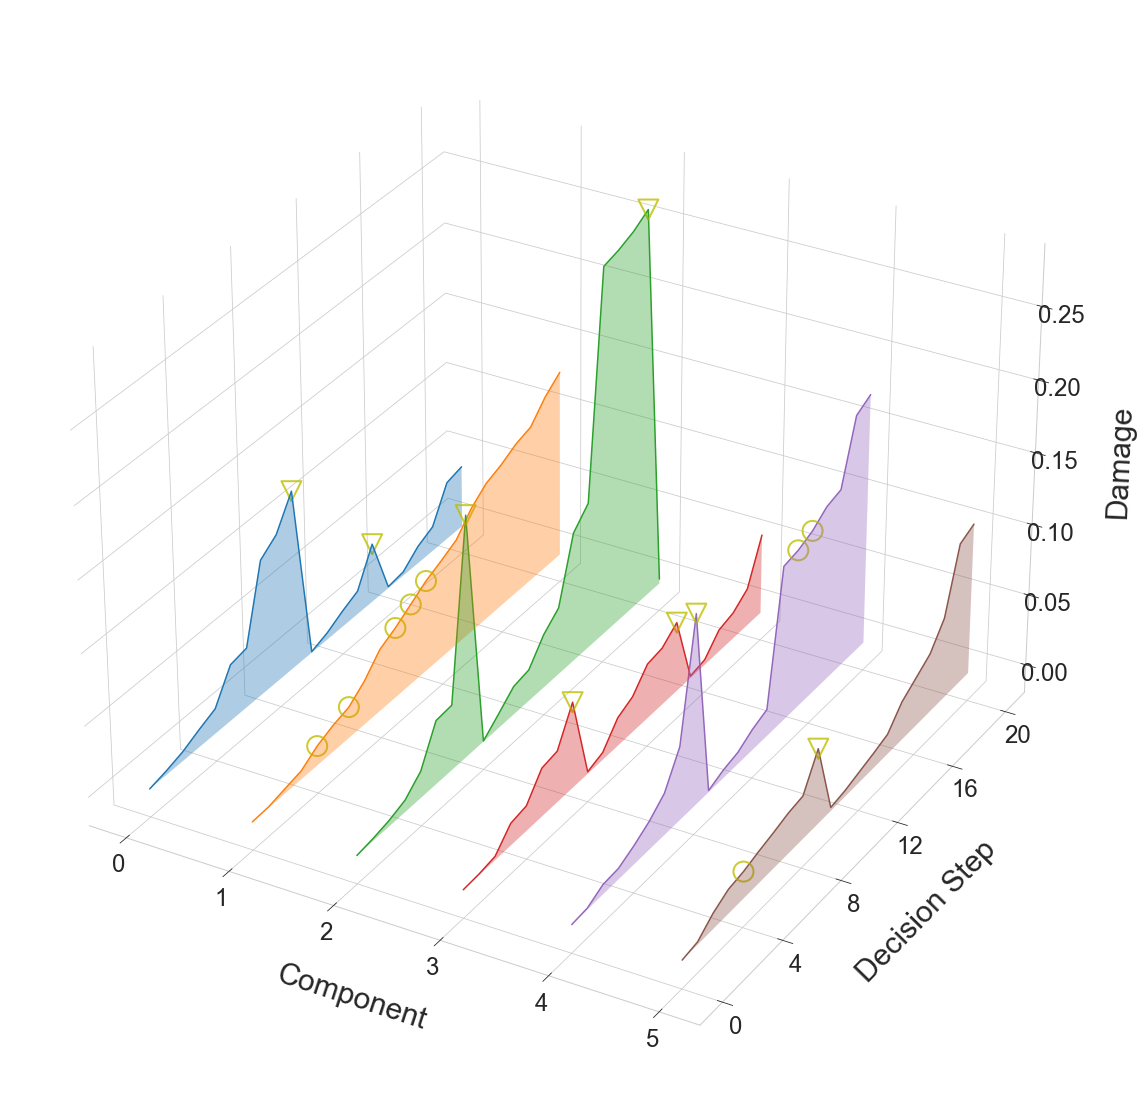
\includegraphics[width=\textwidth]{Figures/allCompsPolReal.png}
	\caption{Policy realization for all components (constrained) - 3D}
	\label{3dPolReal}
\end{figure}

Last but not least, it should be mentioned that the proposed methodology is not strictly applicable only to structural engineering applications. The maintenance of any kind of multi-component engineering system, whose deterioration can be expressed through a stochastic process, can be dealt with using such an approach. Taking advantage of both the capabilities of the \gls{DRL} agent for the sequential decision problem, as well as the more accurate modeling of the deteriorating environment that the continuous variable Bayesian inference provides, renders this framework a promising tool to tackle the problem of maintenance in a general sense.

%------------------------------------------------------------------------------
%	LIMITATIONS
%------------------------------------------------------------------------------

\subsection{Limitations}

As in every research project, there is a trade-off between the modeling accuracy, i.e. the simplifications and assumptions made, and the corresponding computational time. Limiting the assumptions/simplifications for the proposed framework, had the expected outcome regarding the runtime. Therefore, the most important limitation of the developed tool is the high computational time needed for the training of the agent. It makes it significantly difficult to tune the hyper-parameters or do simple modifications to the system's dynamics, which would require the training of the agent from scratch. Nevertheless, it could be characterized as a disadvantage worth having, since such a tool can yield the optimal maintenance strategy for the whole lifetime of an engineering system, making the runtime seem less important on a relative scale. Of course, as displayed also in this thesis, the computational resources needed are proportional to the complexity of the considered system, as the toy problem both in its discrete and continuous version was much faster to solve in comparison with the more complicated case study. A possible solution for this limitation would be the further optimization of the Bayesian inference since it was the least time-efficient part of the algorithm. Additionally, the ever-increasing computational power closely connected with the rapid development of the technology could also help in this aspect in the future.


\newpage

%------------------------------------------------------------------------------
%	FUTURE DEVELOPMENT
%------------------------------------------------------------------------------

\subsection{Future Development} \label{futDev}

The current research investigates the benefits and the potential of a workflow that integrates both \gls{DRL} and \gls{BMU}, aiming to determine the optimal sequence of maintenance decisions. Although the first results of such an approach, which were presented in this thesis, are a promising indicator of its capabilities, many possible additions and modifications can be incorporated into the proposed workflow and would be interesting to examine. These ideas for further development and future research are presented in this section.\\

Regarding the multi-component system that was examined as a case study, there are many possible alternatives as far as the actor network architecture is concerned. The actor network architecture used in this project was a \textit{centralized} one, meaning that there was a single neural network for all the components and all the possible actions (this is explained more thoroughly in Section \ref{caseFrameSec}). A different approach would be to \textit{decentralize} each component's network, in a similar fashion as for \gls{DDMAC} in \cite{andriotis2021deep}. Even though the states remain \textit{centralized} and $s_t$ constitutes the input for every agent, there are as many networks and weights $\theta _i$ as the control points, i.e. the components of the system. This means, each agent chooses an action independently, but they are still aware of one another's condition, owing to the common input they are getting. The described architecture is illustrated in Figure \ref{casePPOnetDecenter}.

\begin{figure}[H]
    \centering
    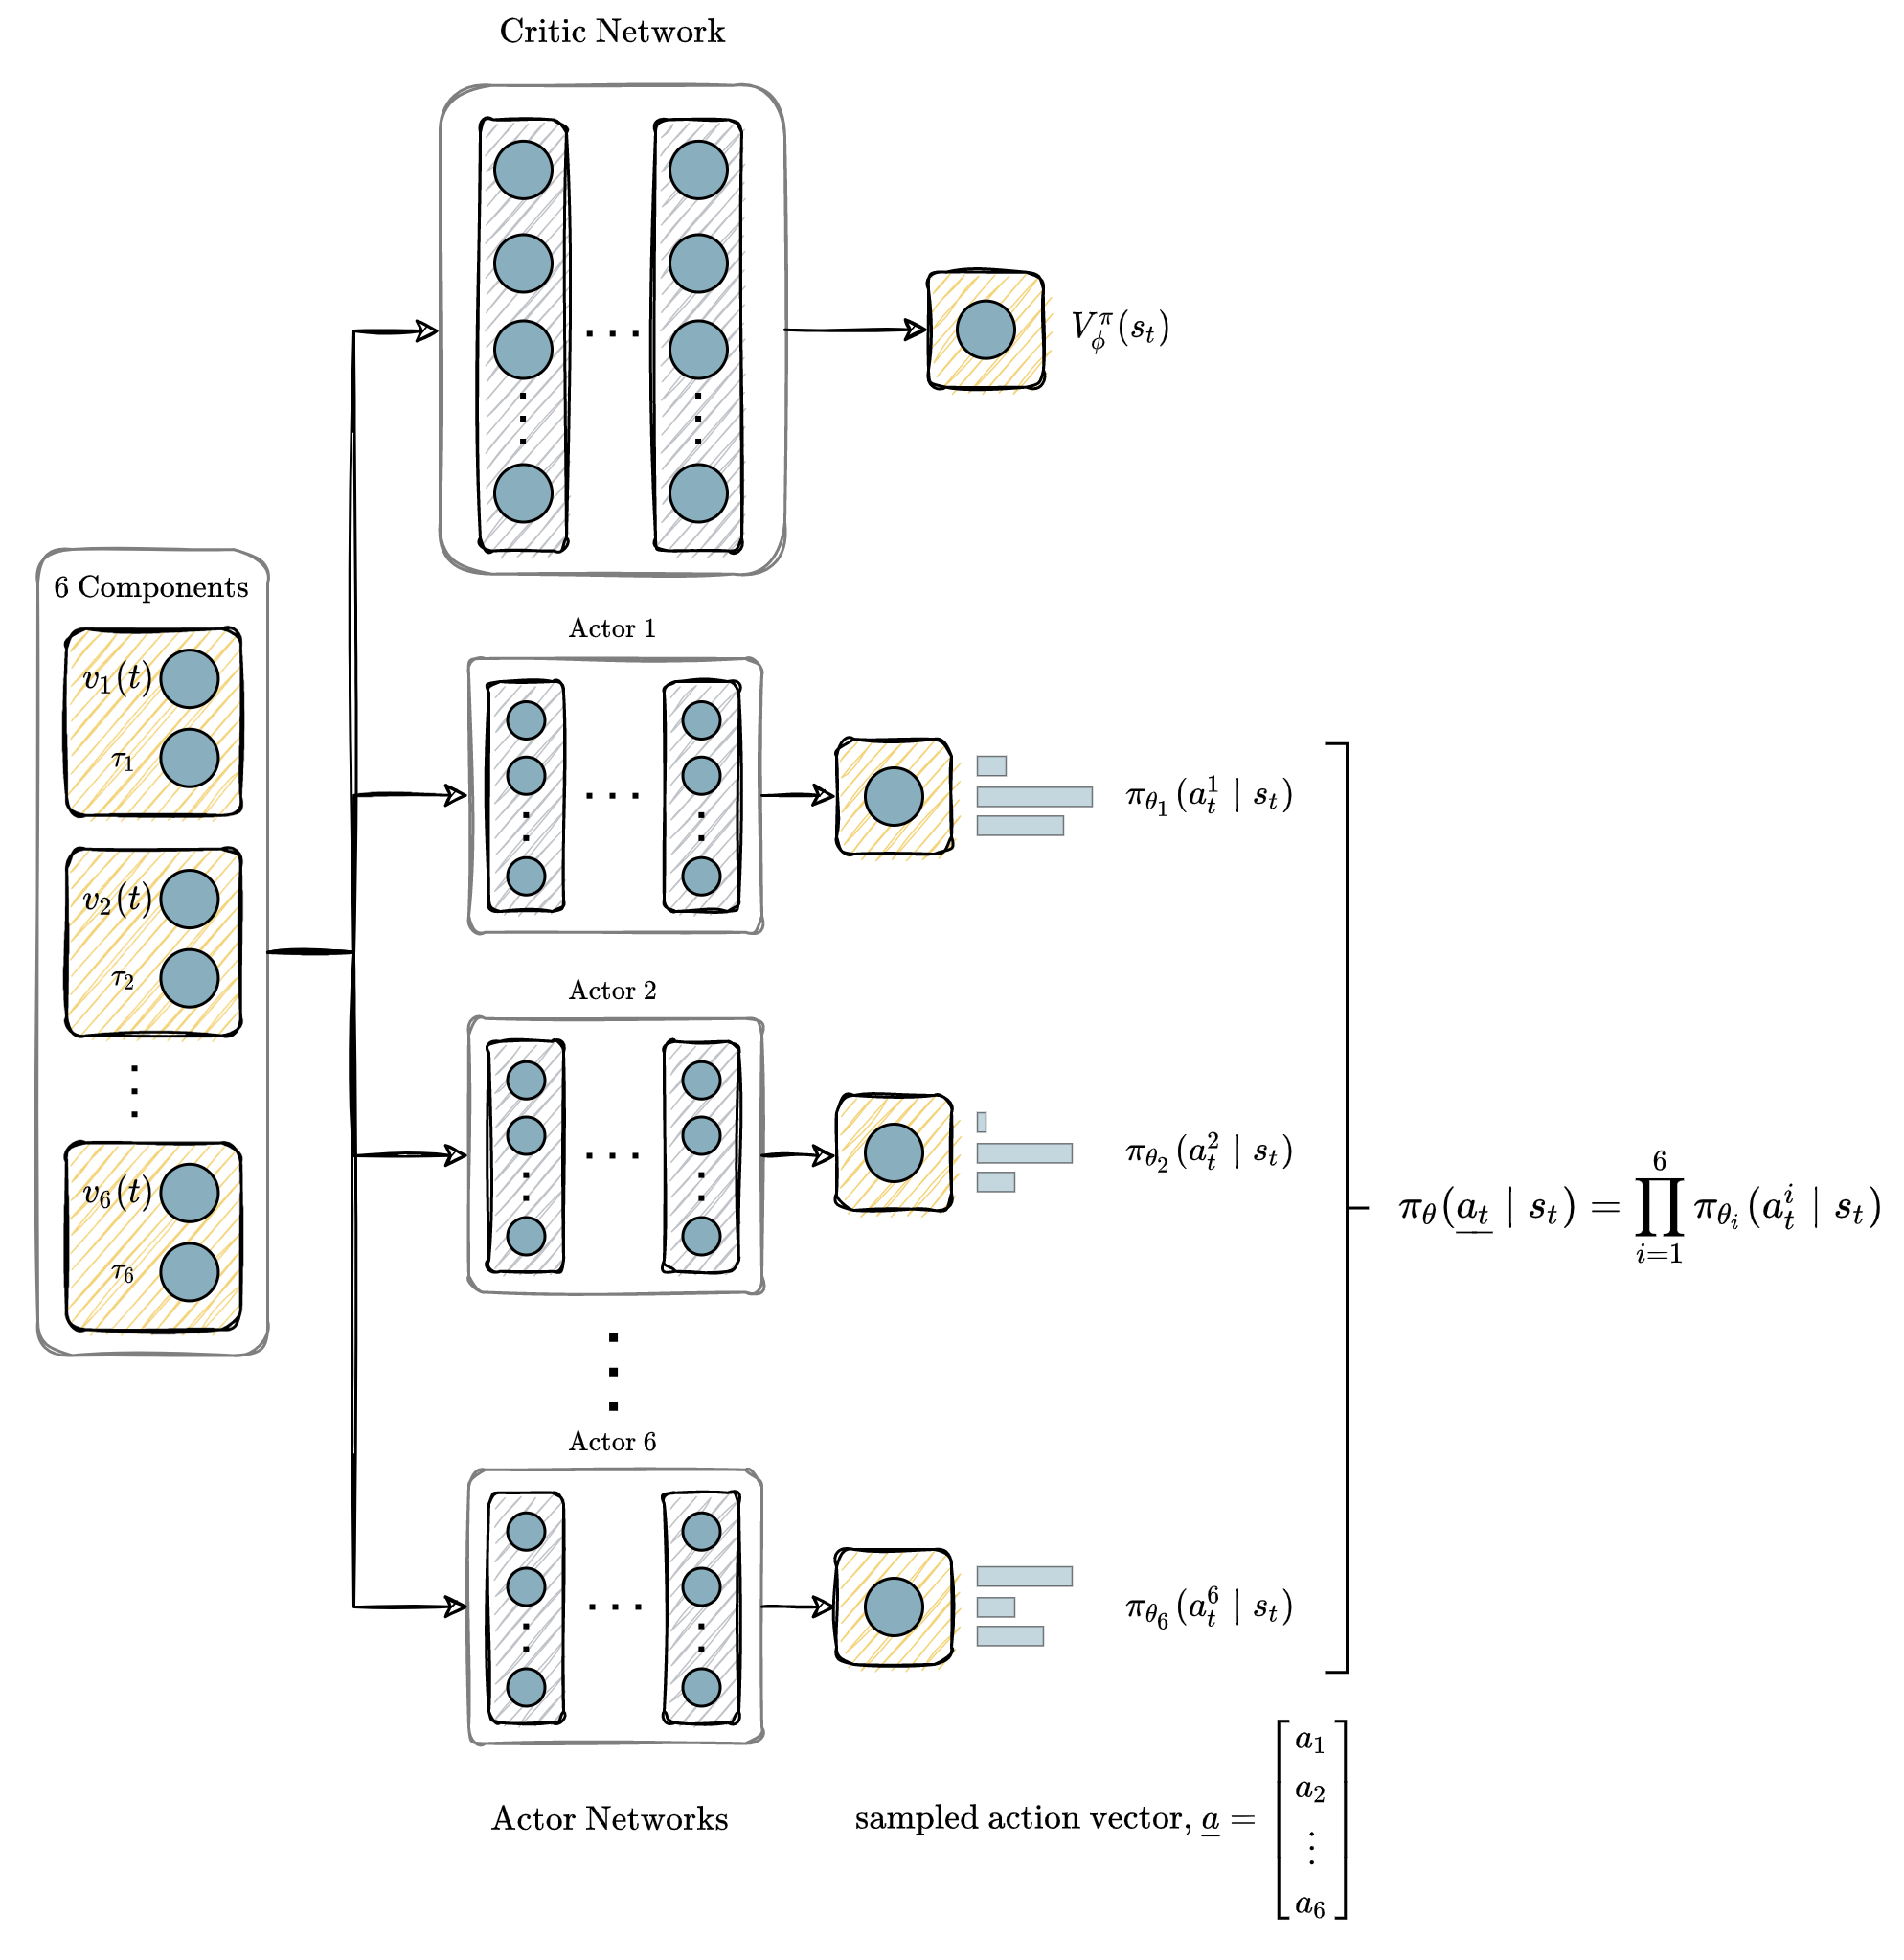
\includegraphics[width=\textwidth]{Figures/neuralNetDecenter.png}
	\caption{\gls{PPO} architecture - Centralized states and decentralized actions}
	\label{casePPOnetDecenter}
\end{figure}

\newpage

A variation of this architecture would be to group the elements that belong to the same floor. From an engineering point of view, it is a valid assumption that columns of the same floor would stochastically be described by a single neural network. Also for this option, the state $s_t$ which contains the damage and the deterioration rate of all components, would be common for all 3 networks (\textit{centralized} states). The output of these \textit{floor} networks would still be a softmax, i.e. $\pi _{\theta_i}$, from which two actions would be sampled (one for each column) during every decision step, as depicted in Figure \ref{casePPOnetPerFloor}. The validity of this proposal can be further backed up if in the case of a \textit{decentralized} 6 sub-network architecture (Figure \ref{casePPOnetDecenter}) the agent chooses eventually symmetrical actions, meaning that similar decisions are made for the columns that belong to the same floor.

\begin{figure}[H]
    \centering
    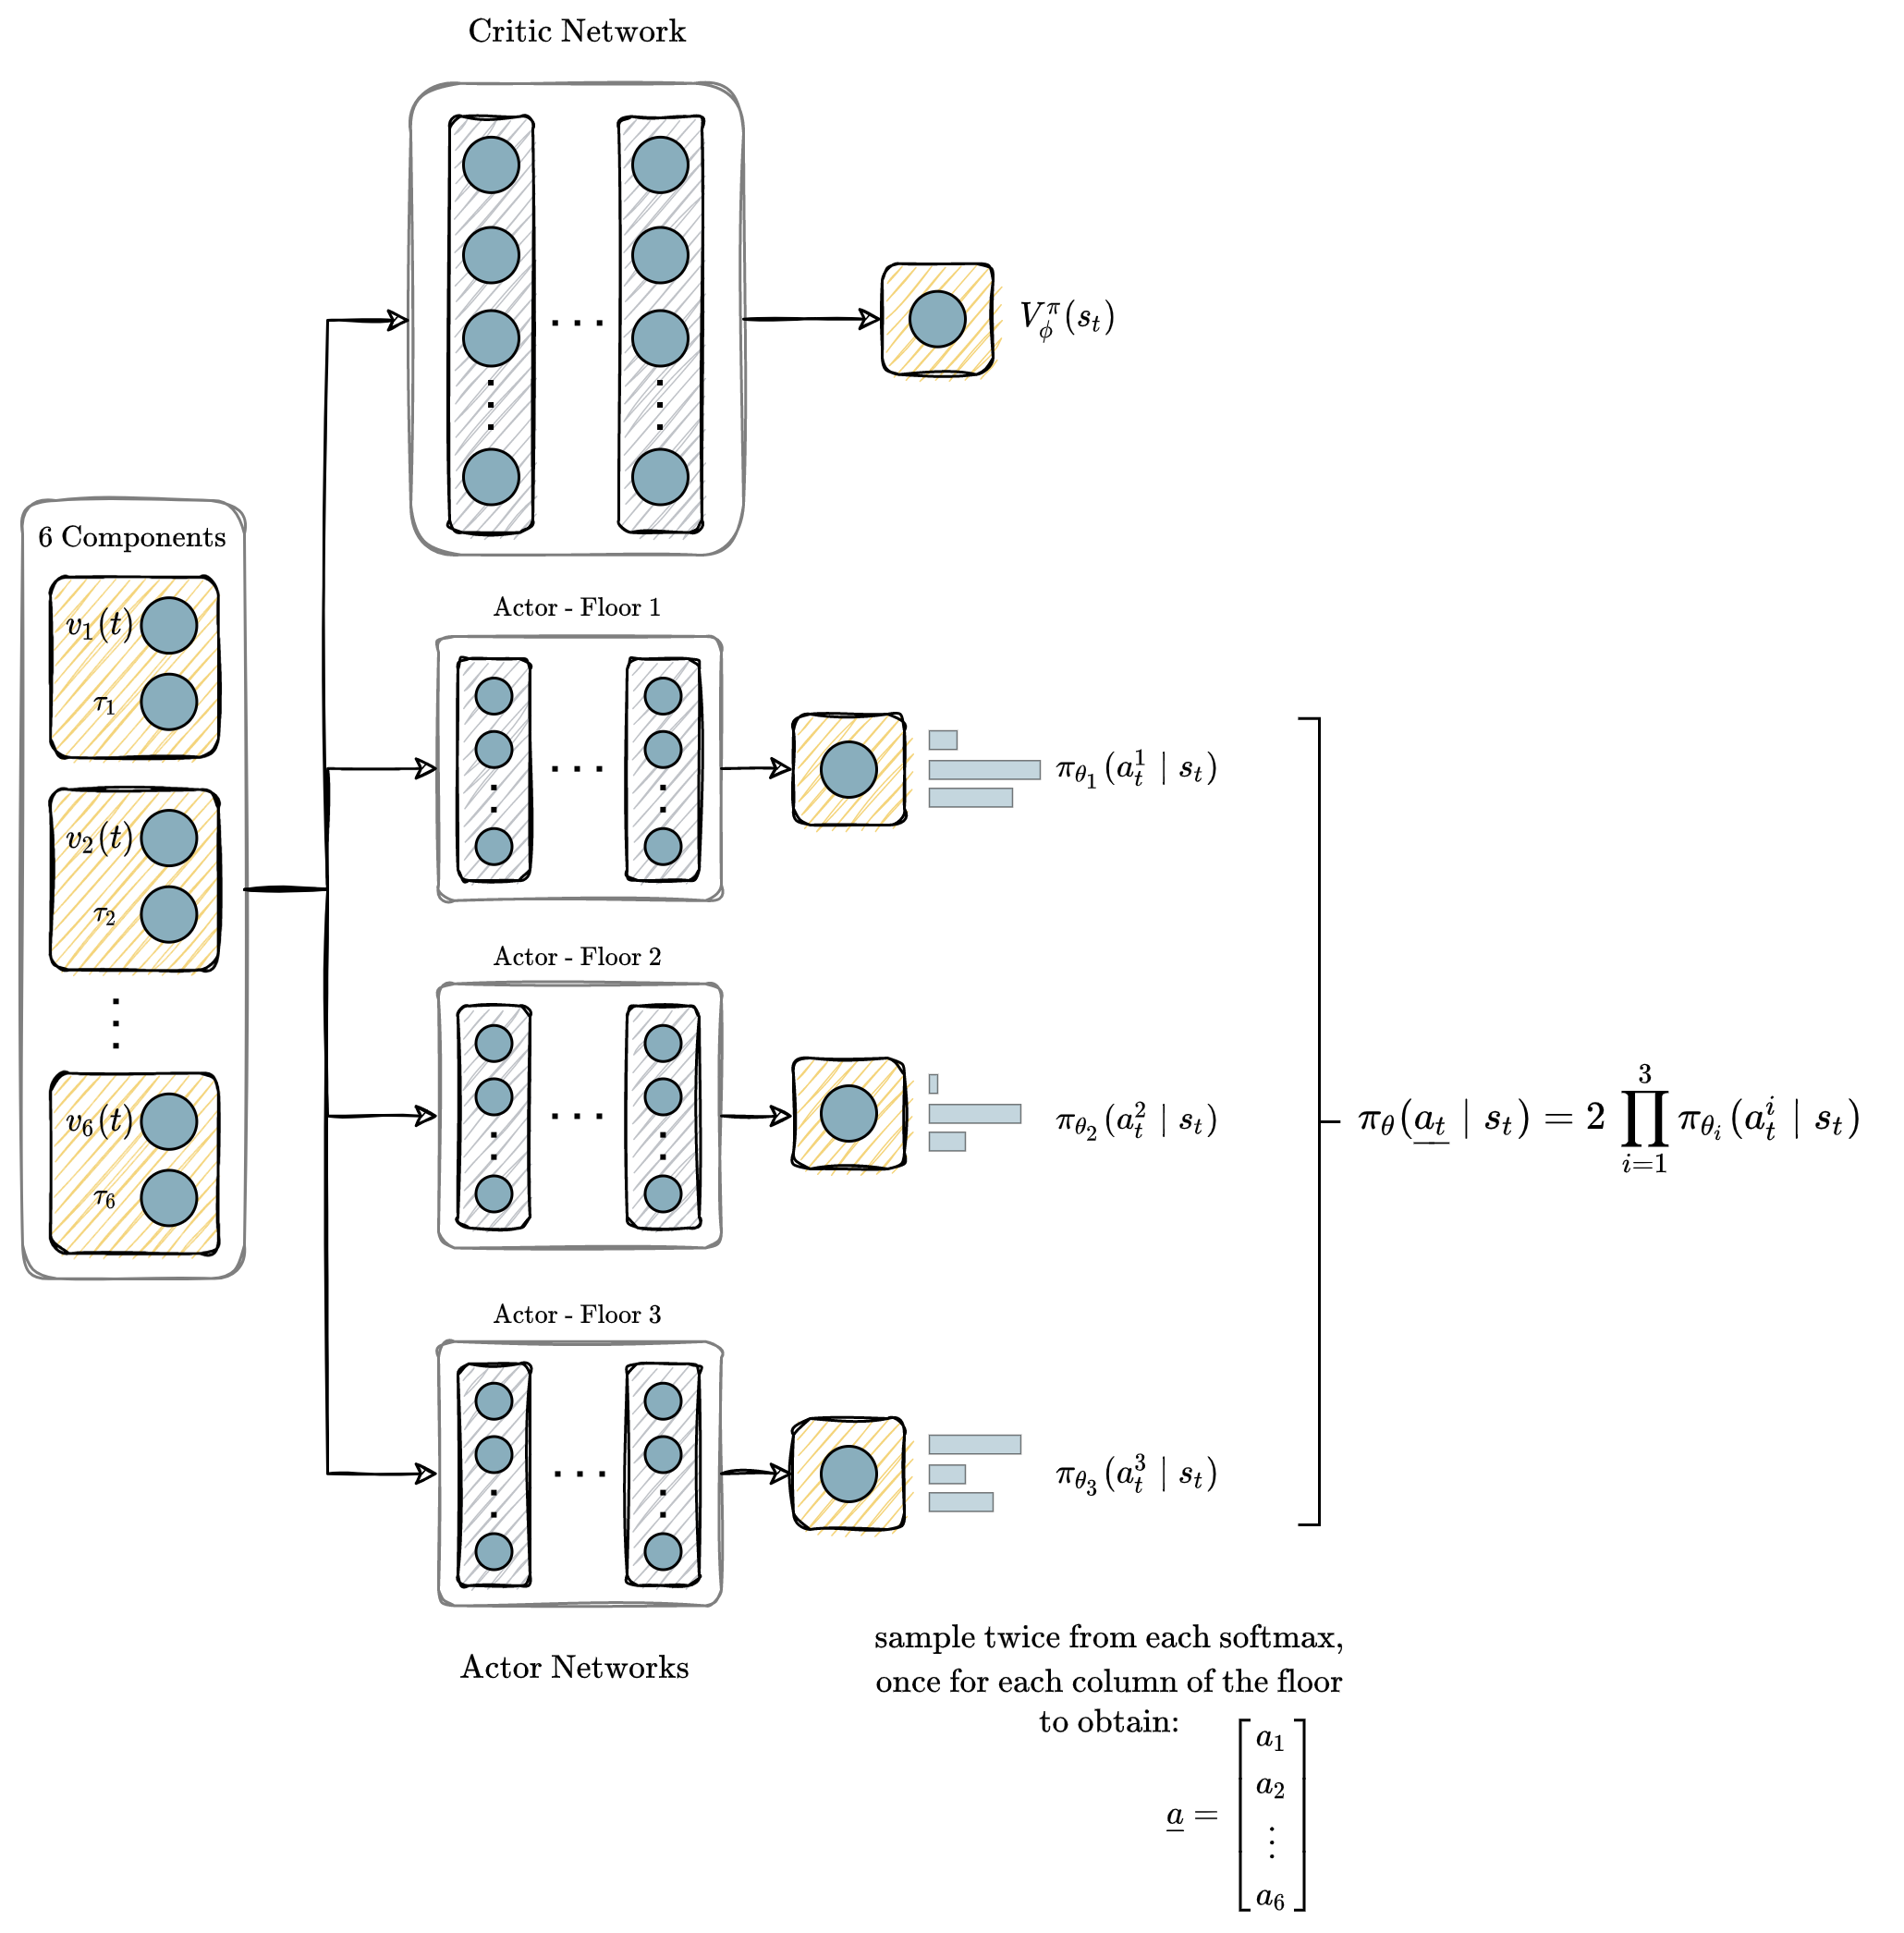
\includegraphics[width=\textwidth]{Figures/neuralNetPerFloor.png}
	\caption{\gls{PPO} architecture - Centralized states and decentralized actions - Floor variation}
	\label{casePPOnetPerFloor}
\end{figure}

\newpage

Lastly, another idea for an actor network architecture would be to consider in the inputs an ID for each component. There will be only one network and shared parameters $\theta$, which would output a single policy $\pi_{\theta}$ with three probabilities which would refer to the component with the given ID. The state $s_t$ containing information for the whole structure will remain as is in the input layer (\textit{centralized} approach), and there will be six 6 forward propagations of the actor network to obtain the six 6 component policies. This idea is depicted in Figure \ref{casePPOnetID}.

\begin{figure}[H]
    \centering
    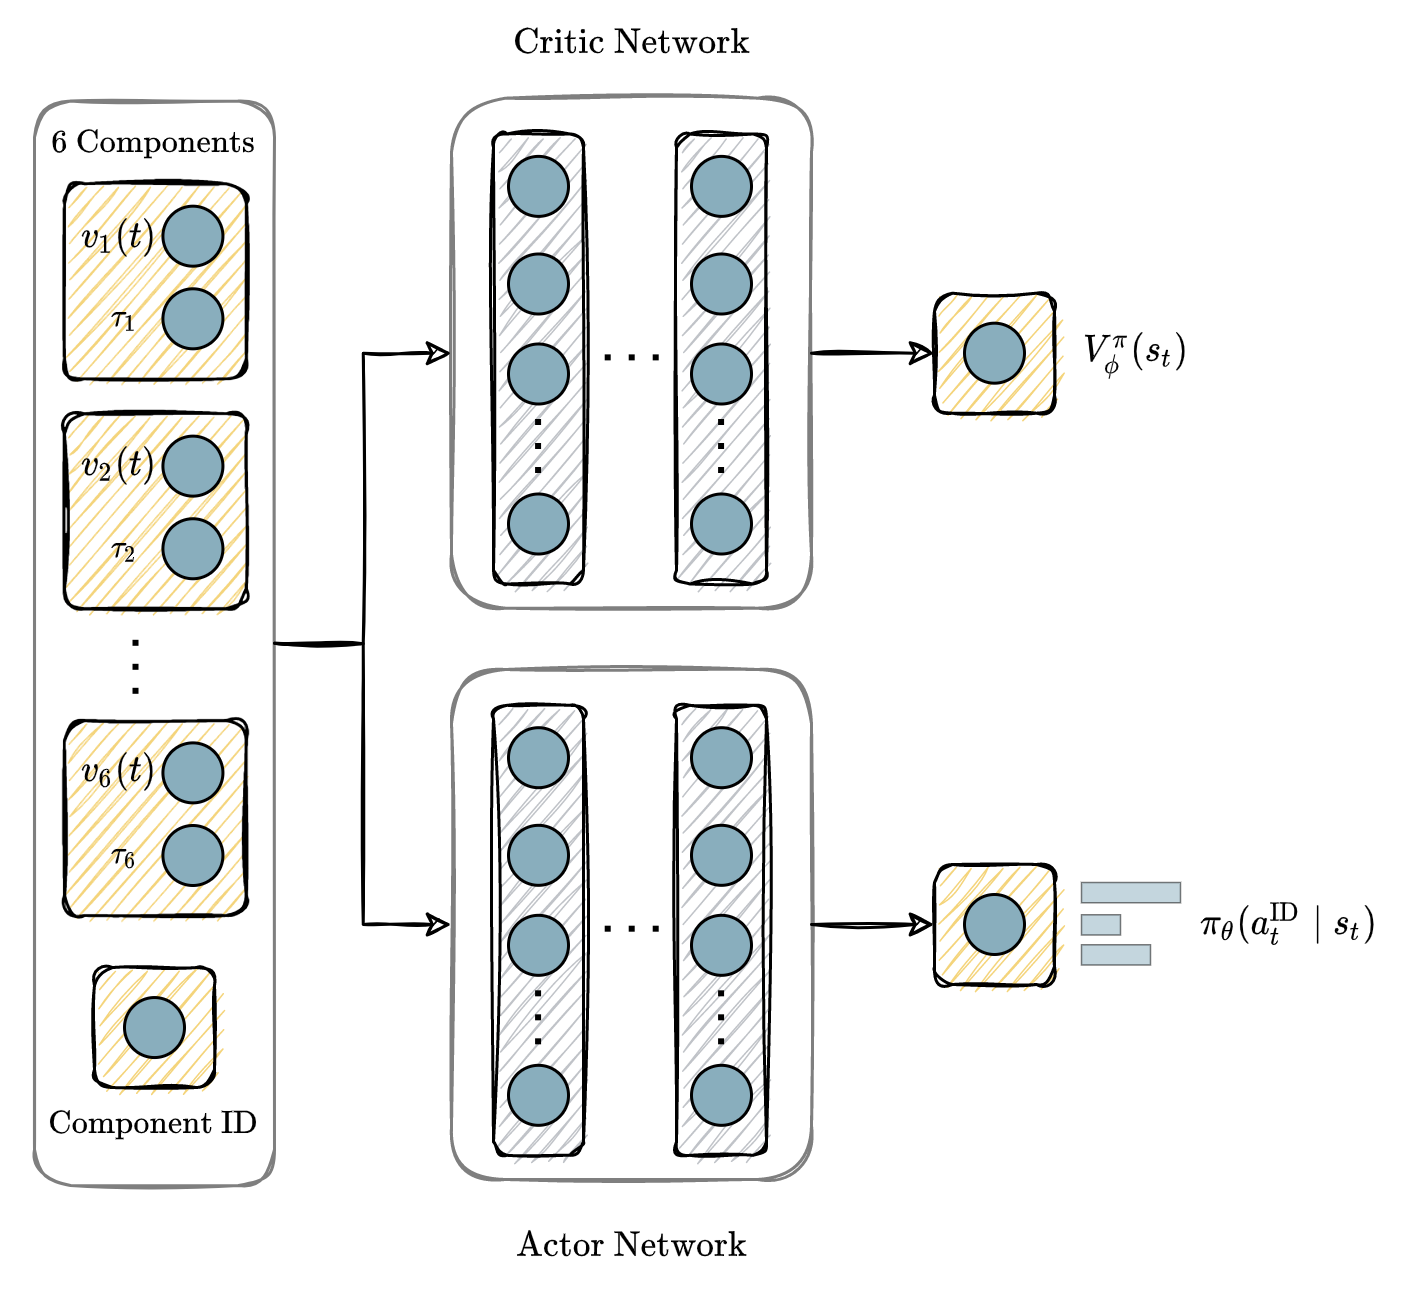
\includegraphics[width=0.8\textwidth]{Figures/neuralNetID.png}
	\caption{\gls{PPO} architecture - Component's ID}
	\label{casePPOnetID}
\end{figure}

\newpage

An interesting idea for a future investigation is the inclusion of the stochastic parameters $A$ and $B$, which are updated in every decision step, to the state $s_t$, hence to the inputs of the neural networks. This modification could lead to the agent making more confident decisions in the later decision steps when it has developed a greater knowledge about the deteriorating environment. Such a feature would also be an important advantage of the proposed methodology in comparison with the traditional approaches, which need to follow a strategy from start to end, and can not capture the decrease of the uncertainties through continuous model updates, subsequently the increase of the decision-maker's confidence.\\

What is more, a worthy addition to this framework would be to account for different/additional actions. One particularly interesting and realistic action scenario would be to reward the grouping of the components' maintenance. More specifically, this can highlight how probable would it be for the agent to choose a single component's action at a higher cost, instead of waiting for other ones to deteriorate further and perform maintenance to more members during the same decision step. This can be modeled using a fixed base cost, e.g. for the maintenance crew to reach the structure's venue, and add to that the cost of the maintenance actions.\\

On a more technical note, currently, \gls{PPO} trains the agent using a rollout buffer, i.e. the stored samples are discarded after their use. Alternatively, to reuse the samples and tackle more efficiently the stochasticity of the problem, a replay buffer can be employed, that will keep the samples even after the training. During the training a weighted sampling can be applied, for the more recent samples (generated by more recent policies) to be more important compared to the old ones (\cite{wang2016sample}, \cite{andriotis2019managing}).\\

Lastly, as already mentioned, the modeling choice of the failure and its corresponding cost, play an important role in the ability of the \gls{DRL} agent to beat the benchmark. To verify this argument, it would be useful to perform a sensitivity analysis for various scenarios of risk of failure cost. Unfortunately, although such runs were initiated for this thesis as well, the computational time was restricting and the proper training of the agent along with hyper-parameter exploration was not possible.


